\section{Theory}
Here is all the theory needed to understand the project.


\subsection{The physical system}
This is the section explaining the physics of the system. 
Throughout the project, \textit{natural units} are used ($\hbar = 1$,$c=1$,$e=1$,$m_e=1$) and all energies are in so-called \textit{atomix units} a.u. 

\subsubsection{The quantum mechanics and the variational principle} \label{sec:quantum_mechanics}

\textbf{The quantum mechanics}

In this project we will look at a system of $N$ electrons in a so-called \textit{quantum dot}.
That is, a two dimensional harmonic oscillator with potential 

\eqs
V(\vec r) = \frac{1}{2} \omega^2 r^2
\label{eq:harmonic_oscillator_potential}
\eqf

This potential gives rise to a multi-particle Hamiltonian $\hat{H}$ given as the sum of an ordinary Hamiltonian and an electron repulsive part

\eqs
\hat{H} = \sum_{i=1}^N \left ( -\frac{1}{2} \nabla_i^2 + \frac{1}{2} \omega^2 r_i^2 \right ) + \sum_{i<j} \frac{1}{r_{ij}} 
\label{eq:harmonic_oscillator_hamiltonian}
\eqf

Where $r_{ij} = |\vec r_i - \vec r_j| $ is the distance between the electrons $i$ and $j$ and $r_i = |\vec r_i | = \sqrt{x_i^2 + y_i^2}$ when $\vec r_i = \left ( \begin{matrix} x_i \\ y_i \end{matrix} \right ) $. 
Our goal in this project is to find the ground eigenstate and energy of this multi-particle Hamiltonian numerically. 

\vspace{0.5cm}
\textbf{The variational principle}

We will approach this by constructing a real test function $\Psi_T(\vec r_0, \vec r_1, ... , \vec r_{N-1}, \alpha,\beta )$ dependent on two parameters $\alpha$ and $\beta$ and calculate the expextation value of the hamilton operator $\langle \hat{H} \rangle $. 
As we know, the eigenstates $\Psi_i$ of the Hamiltonian forms a complete basis, so any state, including our test state $\Psi_T$, can be written as a linear combination of the eigenstates 

\eqs
\Psi_T = \sum_i c_i \Psi_i
\eqf

Inserting this expression into the equation for the expectation value of $\hat{H}$ (remembering that $\Psi_T$ is real) gives

\eqs
\langle \hat{H} \rangle = \frac{\int \Psi_T \hat{H} \Psi_T d\vec r}{ \int \Psi_T \Psi_T d\vec r} = \frac{\int \left ( \sum_i c_i \Psi_i \right ) \hat{H} \left ( \sum_i c_i \Psi_i \right ) d\vec r}{ \int \left ( \sum_i c_i \Psi_i \right ) \left ( \sum_i c_i \Psi_i \right ) d\vec r}
=
\frac{\int \left ( \sum_i c_i \Psi_i \right ) \left ( \sum_i c_i  E_i \Psi_i \right ) d\vec r}{ \int \left ( \sum_i c_i \Psi_i \right ) \left ( \sum_i c_i \Psi_i \right ) d\vec r}
\eqf

The energy of the ground state $E_0$ is smaller than all other $E_i$'s so 

\[
\langle \hat{H} \rangle
=
\frac{\int \left ( \sum_i c_i \Psi_i \right ) \left ( \sum_i c_i  E_i \Psi_i \right ) d\vec r}{ \int \left ( \sum_i c_i \Psi_i \right ) \left ( \sum_i c_i \Psi_i \right ) d\vec r}
\]
\eqs
\geq
\frac{\int \left ( \sum_i c_i \Psi_i \right ) \left ( \sum_i c_i  E_0 \Psi_i \right ) d\vec r}{ \int \left ( \sum_i c_i \Psi_i \right ) \left ( \sum_i c_i \Psi_i \right ) d\vec r}
=
E_0
\frac{\int \left ( \sum_i c_i \Psi_i \right ) \left ( \sum_i c_i  \Psi_i \right ) d\vec r}{ \int \left ( \sum_i c_i \Psi_i \right ) \left ( \sum_i c_i \Psi_i \right ) d\vec r} = E_0
\eqf
\eqs
\langle H \rangle \geq E_0
\eqf

This simple observation is called \textit{the variational principle} and is what we will use to narrow our search for the optimal parameters $\alpha$ and $\beta$.
We will look for the parameters $\alpha$ and $\beta$ that gives us the smallest value of $\langle \hat{H} \rangle$ and this will be our estimate for the ground state.

\vspace{0.5cm}
\textbf{Finding the expectation value of $\hat{H}$}

We have

\eqs
\langle \hat{H} \rangle =  \frac{\int \Psi_T \hat{H} \Psi_T d\vec r}{ \int \Psi_T \Psi_T d\vec r}
=
\int ~\frac{\Psi_T \Psi_T}{\int \Psi_T \Psi_T d\vec r}~ \frac{1}{\Psi_T} \hat{H} \Psi_T d\vec r
\eqf

If we rename probability density function of the particles $\frac{\Psi_T \Psi_T}{\int \Psi_T \Psi_T d\vec r} = P(\vec r)$ and $E_L(\vec r) = \frac{1}{\Psi_T} \hat{H} \Psi_T$, then the integral becomes 

\eqs
\langle \hat{H} \rangle = \int P(\vec r) E_L(\vec r) d\vec r = \langle E_L \rangle
\eqf

But we could very well find a minimum of $\langle \hat{H} \rangle$ that is not an eigen energy of the system, i.e. still larger than $E_0$.
To address this problem, let's look at the variance $V_{E_L}$ of $\langle E_L \rangle$. 

\eqs
V_{E_L} = \langle E_L^2 \rangle - \langle E_L \rangle^2
= 
\int P(\vec r) \left (\frac{1}{\Psi_T} \hat{H} \Psi_T \right )^2 d\vec r -
\left (\int P(\vec r) \frac{1}{\Psi_T} \hat{H} \Psi_T d\vec r \right )^2
\eqf 

If the state $\Psi_T$ is an eigenstate of $\hat{H}$ with eigenvalue $E$ then 

\[
V_{E_L} = \int P(\vec r) \left (\frac{1}{\Psi_T} E \Psi_T \right )^2 d\vec r -
\left (\int P(\vec r) \frac{1}{\Psi_T} E \Psi_T d\vec r \right )^2
\]
\[
=E^2
\left ( 
\int P(\vec r) \left (\frac{1}{\Psi_T} \Psi_T \right )^2 d\vec r -
\left (\int P(\vec r) \frac{1}{\Psi_T} \Psi_T d\vec r \right )^2
\right ) = 
E^2 
\left ( 
\int P(\vec r) (1)^2 d\vec r -
\left ( \int P(\vec r) \cdot 1 d\vec r \right )^2
\right )
\]
\eqs
=
E^2 
\left ( 
\int P(\vec r) d\vec r -
\left ( \int P(\vec r) d\vec r \right )^2
\right ) = E^2 (1-1^2) = 0
\eqf

So if $\Psi_T$ is an eigenstate of $\hat{H}$ then the variance $V_{E_L}$ of $E_L$ is $0$

\eqs
V_{E_L} = \langle E_L^2 \rangle - \langle E_L \rangle^2 = 0
\eqf 

This will serve as a verification that the state we have found when minimizing the expectation value of $E_L$ is indeed an eigenstate of the hamilton operator. 










\subsubsection{The test function $\Psi_T$}

We will in this project use the trial wavefunctions of $\vec r_i = \left ( \begin{matrix} x_i \\ y_i \\ \end{matrix}\right )$

\eqs
\Psi_T(\vec r_0, ... ,\vec r_{N-1})  = \Det(\phi_1,  ... , \phi_N) \cdot \textrm{J}(\vec r_0, ... , \vec r_{N-1} )
\eqf

Where $\textrm{J} (\vec r_0, ... , \vec r_{N-1} )$ is a so-called \textit{Jastrow factor}, which represents the electron repulsion part of the wavefunction, defined as

\[
\textrm{J}(\vec r_0, ... \vec r_{N-1}) = \prod_{i<j}^N \exp \left (
\frac{a_{ij}r_{ij}}{1 + \beta r_{ij}}
\right ) 
\quad
\textrm{where}
\]
\eqs
\quad
r_{ij} = |\vec r_i - \vec r_j  \quad \textrm{and} 
\quad 
a_{ij} = \left \{
\begin{matrix}
1/3  & \textrm{if spin(i) and spin(j) are parallell} \\
1  & \textrm{if spin(i) and spin(j) are anti-parallell} \\
\end{matrix}
\right .
\eqf


$\Det(\phi_0,  ... , \phi_{N-1})$ is the \textit{Slater determinant} defined as 

\eqs
\Det(\phi_1,  ... , \phi_N) = \frac{1}{\sqrt{N!}} \left |
\begin{matrix}
\phi_0(\vec r_0) & \phi_1(\vec r_0) & ... & \phi_{N-1}(\vec r_0) \\
\phi_0(\vec r_1) & \phi_1(\vec r_1) & ... & \phi_{N-1}(\vec r_1) \\
       ...          &      ...       & ... & ... \\
\phi_0(\vec r_{N-1}) & \phi_1(\vec r_{N-1}) & ... & \phi_{N-1}(\vec r_{N-1}) \\
\end{matrix}
\right |
\eqf

$\phi_i(\vec r_i)$ is a wavefunction resembling one of the eigenfunctions of the Hamilton operator for \textit{one} particle in a two dimensional harmonic oscillator, but parameterized by $\alpha$ in the following way:

\eqs
\phi_i(\vec r_j) = H_{n_x} (\sqrt{\alpha \omega} x_j) H_{n_y} (\sqrt{\alpha \omega} y_j) \exp(-\alpha \omega (x^2 + y^2)/2) 
\eqf


Where $n_x(i)$ and $n_y(i)$ corresponds to the quantum numbers needed to "fill up" the system from the lowest energy levels twice (one for each spin configuration). 
For $i<12$, the explicit depence of $n_x, n_y$ on $i$ is given in table \ref{tab:dependence_of_nx_on_i}.


\begin{table}[h!]
	\centering
	\begin{tabular}{lllllllllllll}
	\toprule 
	$ i = $ & 0 & 1 & 2 & 3 & 4 & 5 & 6 & 7 & 8 & 9 & 10 & 11 \\
	\midrule
	$n_x = $ & 0 & 0 & 1 & 1 & 0 & 0 & 2 & 2 & 1 & 1 & 0 & 0 \\
	$n_y = $ & 0 & 0 & 0 & 0 & 1 & 1 & 0 & 0 & 1 & 1 & 2 & 2 \\
	\bottomrule
	\end{tabular}
	\caption{The explicit dependence of $n_x$ and $n_y$ on $i$ in the construction of the trial wavefunctions.}
	\label{tab:dependence_of_nx_on_i}
\end{table}


It can be shown \cite{master} that. 
















\subsubsection{Discretization}

\subsubsection{The virial theorem}


\subsection{The numerical foundation}
This is the section explaining the numerical theory upon which the project is built. 

\subsubsection{Monte Carlo simulations}
A Monte Carlo simulation is a way of solving a mathematical or physical problem by generating a random
(or pseudorandom
\footnote
{No electronic random number generator of today is truly random. 
The sequence of numbers generated will repeat itself after a long period. 
These periods however, are increadibly long and we will for this report 
consider the random number generators to be truly random.})
sequence of numbers and evaluating some quantity on the assumption that our the random sequence of numbers is representative of the domain from which the quantity is evaluated.
An example is evaluating the area of the unit circle by randomly placing points in a $[-1,1] \times [-1,1] $ grid and find the fraction points whose distance to the origin is $\leq 1$ and multiply this fraction by the area of the grid (i.e. $4$).
Such a simple Monte Carlo simulation can give the result as shown in figure \ref{fig:Monte_Carlo_Illustration}.

\begin{figure}[h!]
        \centering 
        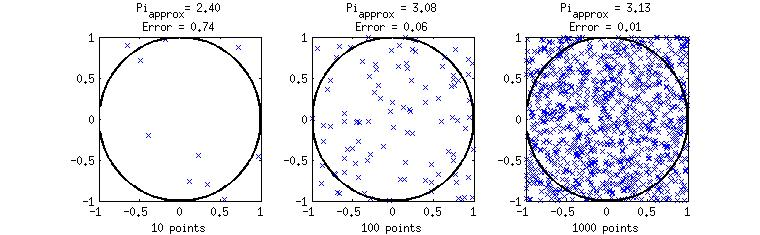
\includegraphics[width=\textwidth]{Monte_Carlo_Illustration.jpg}
        \caption{The results from a very simple Monte Carlo simulation of 
        estimating the circle constant $\pi$. 
        The precision increases with the number of points.}
        \label{fig:Monte_Carlo_Illustration}
\end{figure}

However, the method is not confined to this sort of problem, but can be applied to a variety of mathematical and physical problems. 
In this report, the method, through the Metropolis algorithm (see section \ref{sec:theory_metropolis}) has been applied to a quantum mechanical system.

\subsubsection{Importance sampling}

Sometimes, functions are more important in certain domains.
When we use a Monte Carlo approach to evaluate a quantity on such a function we can improve the method significantly by ensuring that the probability distribution from which we choose our random values reflect the parts where the function is important.
We do of course have to remember that our function lives on its whole domain, so to not get a biased result, we need to weigh our result with respect to the probability function we have chosen. 
This is called importance sampling. 
\textbf{INSERT EXAMPLE HERE}

\subsubsection{The Metropolis algorithm} \label{sec:theory_metropolis}

The Metropolis algorithm is a method which cleverly employs a stoichastic approach in order to quickly estimate certain mathematical objects.
The method is explained at lengths elsewhere\cite{lecturenotes}, but in this section we will look at an example which captures the main idea of the method.

Suppose we have a PDF\footnote{Probability Distribution Function} $P(x)$ in a domain $[a,b]$ for which we want to calculate the expectation value $\langle g \rangle$ of some function $g(x)$. 
The integral we need to solve is then 

\eqs
\langle g \rangle = \int_a^b P(x) g(x) dx 
\eqf

This integral can be approximated as follows

\eqs
\int_a^b P(x) g(x) dx \approx \frac{b-a}{N} \sum_i P(x_i) g(x_i) \equiv I 
\eqf

Where $x_i$ are some uniformly chosen values in the interval $[a,b]$. 
Now, imagine instead of picking values $x_i$ uniformly and weighing them by multiplying $g(x)$ with $P(x)$ instead chose the values of $\tilde{x_i}$ from the PDF $P(x)$ and calculated the quantity $\tilde{I}$ given by

\eqs
\tilde{I} = \frac{1}{N} \sum_i g(\tilde{x_i})
\label{eq:metropolis_integral}
\eqf

It can be shown mathematically that for large enough $N$, these two quantities $I$ and $\tilde{I}$ approach the same value.  
The problem with such an approach is that we need the precise expression for the PDF $P(x)$ and a robust algorithm for choosing random values from it. 
With the Metropolis algorithm however, we can use this approach \textit{without} knowing the precise expression of the PDF and the relevant values from the domain come naturally. 

The algorithm requires that we are able to calculate $\tilde{P}(x)$, an unnormalized version of $P(x)$ (i.e. some function $aP(x)$ proportional to $P(x)$). 
This may seem like a very strong requirement, but in many applications, as in this project, this is a much easier task than to calculate the precise PDF. 
The algorithm goes as follows. 
Starting with a position $x$ choose a new trial position 

\eqs x_p = x + r \Delta x \eqf

Where $\Delta x$ is a predefined step length and $r$ is a random number between zero and one. 
Then generate a probability criteria $s$, a random number between zero and one. 
If 

\eqs \frac{P(x_p)}{P(x)} = \frac{aP(x_p)}{aP(x)} = \frac{\tilde{P}(x_p)}{\tilde{P}(x)} \equiv w \geq s 
\label{eq:metropolis_prob_crit}\eqf

We accept the trial position as our new $x$ and if not we reject it. 
If we choose new values of $x_i$ in this manner, the collection of $x_i$'s will in fact reflect the PDF $P(x)$, which was what we needed in order to use equation \ref{eq:metropolis_integral}. 
Note how equation \ref{eq:metropolis_prob_crit} doesn't require us to have the exact form of the probability distribution function, only a function $\tilde{P}(x)$ proportional to it. 

The intuition behind the algorithm is that for each new position $x_i$ we generate is drawn towards the part of the domain where $P(x)$ is bigger. 
To see this, we note that if $P(x_p) > P(x)$ then $\frac{P(x_p)}{P(x)}>1$ which is always bigger than $s \in [0,1]$ and the new move is always accepted.
Whereas if $P(x_p)<P(x)$, the move might be rejected. 
This allows new values of $x_i$ to be chosen from where $P(x)$ is big, but at the same time allows values with lower values of $P(x)$ to be chosen. 
Which is what we expect from a PDF. 
The fact that for a large number $M$ of such steps, the values $x_i$ picked actually reflects the PDF requires some more mathematics, and once again we refer to the lecture notes of the course \cite{lecturenotes}.

As discussed in section \ref{sec:quantum_mechanics} we need to solve the integral 

\eqs \langle E_L \rangle = \int P(\vec r) E_L(\vec r) d\vec r \eqf

Where we have a trial function 

\eqs \Psi_T(\vec r_0 ,..., \vec r_{N-1},\alpha,\beta) \eqf

dependent on 2 trial parameters $\alpha$ and $\beta$
where $\vec r_i = \left ( \begin{matrix} x_i \\ y_i \\ \end{matrix} \right )$.
This is exactly the kind of problem the Metropolis algorithm can solve and the explicit algorithm for calculating $\langle E_L \rangle$ and $\langle E_L^2 \rangle$ is given in algorithm \ref{alg:metropolis}.

\begin{algorithm}[h!]
\DontPrintSemicolon
\KwData{\;
An initial position matrix $\mathbf{r} = (\vec r_0, \vec r_1 ... \vec r_{N-1})
=
\left (
\begin{matrix}
x_0 & x_1 & ... & x_{N-1}\\
y_0 & y_1  & ... & y_{N-1}\\
\end{matrix}
\right )$ \;
A method of chosing the step $ \quad \textrm{Method}(\textbf{r}) = \Delta \vec r = \left ( \begin{matrix} \Delta x \\ \Delta y \\ \end{matrix}  \right ) $ \;}
\KwResult{\;
The expectation value of the local energy: $\langle E_L \rangle$ \;
The expectation value of the local energy squared: $\langle E_L^2 \rangle$ \;}
\Begin{
\
$\textit{cumulative\_local\_energy} = 0$ \tcp*{Initialization}
$\textit{cumulative\_local\_energy\_squared} = 0$ \;
$\textit{counter} = 0$\;
\While{$\textit{counter} < M$ }{
        $i = \textrm{randint(} 0,1,...,N-1)$ \tcp*{Choose random element index}
        $\Delta \vec r = \textrm{Method}(\mathbf{r})$
        \tcp*{Create a random two-dimensional step}
        $\mathbf{r_p} = \left ( 
        \begin{matrix} x_0 \\ y_0  \end{matrix} ~
        \begin{matrix} x_1 \\ y_1  \end{matrix} ~
        ... ~~
        \begin{matrix} x_i \\ y_i  \end{matrix} + \Delta \vec r ~~
        ... ~
        \begin{matrix} x_{N-1} \\ y_{N-1}  \end{matrix} ~
        \right ) $ \tcp*{Create a trial position matrix}
        $ s = \textrm{randint(0,1)}$ \tcp*{Generate a probability criteria}
        $w = |\psi(\alpha,\beta,\mathbf{r_p})|^2/
        |\psi(\alpha,\beta,\mathbf{r})|^2$ \tcp*{Calulate the probability ratio}
        \If{$w\geq s$}{
                $\vec r = \vec r_p$ \;
                $E_L(\mathbf{r}, \alpha, \beta) = 
                \frac{1}{\Psi_T(\mathbf{r}, \alpha, \beta)} 
                \hat{H} \psi_T(\mathbf{r},\alpha,\beta)$ \tcp*{Calculate the local energy }
                $\textit{cumulative\_local\_energy}~~ ^+_= ~~E_L(\mathbf{r}, \alpha, \beta)$ \tcp*{Update $\textit{cumulative\_local\_energy}$}
                $\textit{cumulative\_local\_energy\_squared}~~ ^+_= ~~E_L(\mathbf{r}, \alpha, \beta)^2$ \\ \tcp*{Update $\textit{cumulative\_local\_energy\_squared}$}
                $\textit{counter}~ ^+_= ~1$ \tcp*{Update \textit{counter}} 
        }       
 }
Calculate $\langle E_L \rangle = \frac{\textit{cumulative\_local\_energy}}{M}$ \;
Calculate $\langle E_L^2 \rangle = \frac{\textit{cumulative\_local\_energy\_squared}}{M}$ \;
}
\caption{The metropolis algorithm used for finding the expecation value of the
local energy and the expecation value of the local energy squared.}
\label{alg:metropolis}
\end{algorithm}




